\documentclass[journal]{IEEEtran}
\usepackage{cite}
\usepackage{amsmath,amssymb,amsfonts}
\usepackage{algorithmic}
\usepackage{graphicx}
\usepackage{textcomp}
\usepackage{xcolor}
\usepackage{booktabs}
\begin{document}

\title{Taller 1: Regresión Lineal y Regresión Logística sobre el Paddy Dataset}
\author{Salomón Avila, Carlos Caicedo
\thanks{}}
\maketitle

\begin{abstract}
Este documento presenta el desarrollo del Taller 1 de la Maestría en Inteligencia Artificial, curso de Aprendizaje de Máquina. Se implementan desde cero, utilizando únicamente NumPy para los cálculos vectorizados, un modelo de regresión lineal (Punto 1) y un modelo de regresión logística (Punto 2) sobre el conjunto de datos Paddy Dataset de UCI Machine Learning Repository.
\end{abstract}

\begin{IEEEkeywords}
Regresión lineal, Regresión logística, Descenso de gradiente, NumPy, Regularización L2, Paddy Dataset
\end{IEEEkeywords}

%======================================================================
% ===================== PUNTO 1 =========================
%======================================================================
\section{Punto 1: Regresión Lineal}

\subsection{Exploración de datos}

La variable objetivo \texttt{Productividad} no existe en el dataset original. Se construye dividiendo el rendimiento total entre las hectáreas cultivadas:

\begin{equation}
\text{Productividad} = \frac{\text{Paddy yield}}{\text{Hectares}}
\label{eq:productividad}
\end{equation}

Una vez calculada, la columna \texttt{Paddy yield} se elimina del conjunto de variables predictoras, ya que la propia definición de la variable objetivo depende de ella de forma determinista. La distribución de \texttt{Productividad} muestra una desviación estándar pequeña frente a su media, lo que anticipa que el margen de mejora frente a una predicción constante es limitado.

\subsubsection{Correlación de Pearson}
Para orientar la selección de variables se calcula la correlación entre cada variable numérica y la productividad. A diferencia de una simple llamada a una función de una librería, el coeficiente se implementa desde cero de forma vectorizada con NumPy, siguiendo su definición matemática:

\begin{equation}
r = \frac{\sum_i (x_i-\bar{x})(y_i-\bar{y})}{\sqrt{\sum_i (x_i-\bar{x})^2}\sqrt{\sum_i (y_i-\bar{y})^2}}
\label{eq:pearson}
\end{equation}

\begin{figure}[h]
    \centering
    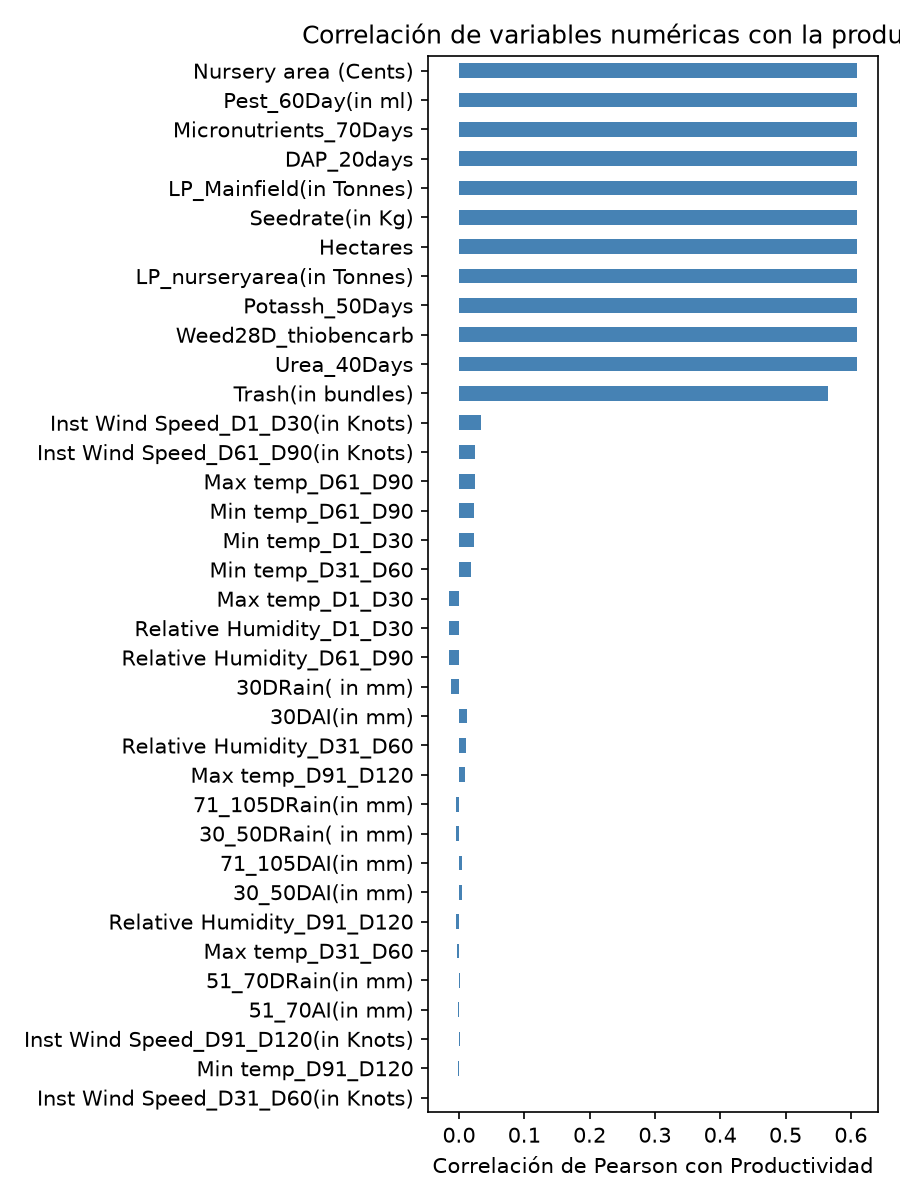
\includegraphics[width=\columnwidth]{correlacion_productividad.png}
    \caption{Correlación de Pearson de las variables numéricas con la variable objetivo Productividad.}
    \label{fig:correlacion_productividad}
\end{figure}

\subsubsection{Identificación de variables redundantes}
Un grupo de diez variables agronómicas presenta exactamente la misma correlación con la productividad, lo que resulta sospechoso. Para confirmar que se trata de copias redundantes de \texttt{Hectares} bajo otra escala, se calcula la desviación estándar de la razón entre cada variable y \texttt{Hectares}. El resultado es una correlación de $1.0$ frente a \texttt{Hectares} y una desviación estándar de $0.0$ en dicha razón para las diez variables, lo que demuestra matemáticamente que corresponden a transformaciones lineales deterministas de \texttt{Hectares}. En consecuencia se descartan estas diez variables, conservando únicamente \texttt{Hectares} como representante del grupo.

Adicionalmente, \texttt{Trash} muestra una correlación de $0.56$ con la productividad y de $0.96$ con el rendimiento total, muy por encima del resto de las variables climáticas y agronómicas. Siguiendo el mismo criterio de descartar variables con correlación extremadamente alta frente al resto, se elimina \texttt{Trash} del conjunto de predictores.

\subsubsection{Transformación de variables}
Las variables categóricas nominales, incluida la dirección del viento en cada ventana de tiempo, se convierten a variables dummy mediante codificación one hot, eliminando una categoría de referencia por variable para evitar colinealidad perfecta con el término de sesgo.

\subsection{Partición de datos}
El dataset se particiona en tres subconjuntos, utilizando \texttt{random\_state=200} para garantizar reproducibilidad:
\begin{itemize}
    \item \textbf{Train (70\%):} para ajustar los parámetros $\theta$.
    \item \textbf{Validation (15\%):} para comparar hipótesis e hiperparámetros y seleccionar el modelo.
    \item \textbf{Test (15\%):} para estimar el error final sobre datos no vistos, utilizado únicamente al final.
\end{itemize}

\subsection{Implementación del modelo}
Se implementa un modelo de regresión lineal múltiple con descenso de gradiente por lotes, función de costo MSE y regularización L2. La hipótesis del modelo es:

\begin{equation}
\hat{y} = X\theta
\label{eq:hipotesis_lineal}
\end{equation}

donde $X$ incluye la columna de sesgo. La función de costo regularizada, con el término de penalización escalado por $m$, el número de variables sin contar el sesgo, es:

\begin{equation}
J(\theta) = \frac{1}{2n}\sum_{i=1}^{n} (x_i^\top\theta - y_i)^2 + \frac{1}{2m}\lambda\sum_{j=1}^{m}\theta_j^2
\label{eq:mse_reg}
\end{equation}

y el gradiente correspondiente es:

\begin{equation}
\nabla J(\theta) = \frac{1}{n}X^\top(X\theta-y) + \frac{\lambda}{m}\theta
\label{eq:grad_lineal}
\end{equation}

sin aplicar la penalización al término de sesgo $\theta_0$. Los parámetros se actualizan mediante:

\begin{equation}
\theta := \theta - \alpha\nabla J(\theta)
\label{eq:update_lineal}
\end{equation}

Antes de estandarizar, las variables numéricas presentan escalas muy distintas entre sí, por lo que el descenso de gradiente diverge si se aplica directamente sobre los datos crudos. Por ello cada variable se estandariza restando la media y dividiendo por la desviación estándar del conjunto de entrenamiento, y esos mismos estadísticos se reutilizan sobre validación y test.

\subsubsection{Verificación de la implementación}
Antes de experimentar con el modelo completo, se verifica que el descenso de gradiente reduce la función de costo de forma monótona en un caso simple, entrenando durante 2000 épocas con $\alpha=0.1$ sin regularización.

\begin{figure}[h]
    \centering
    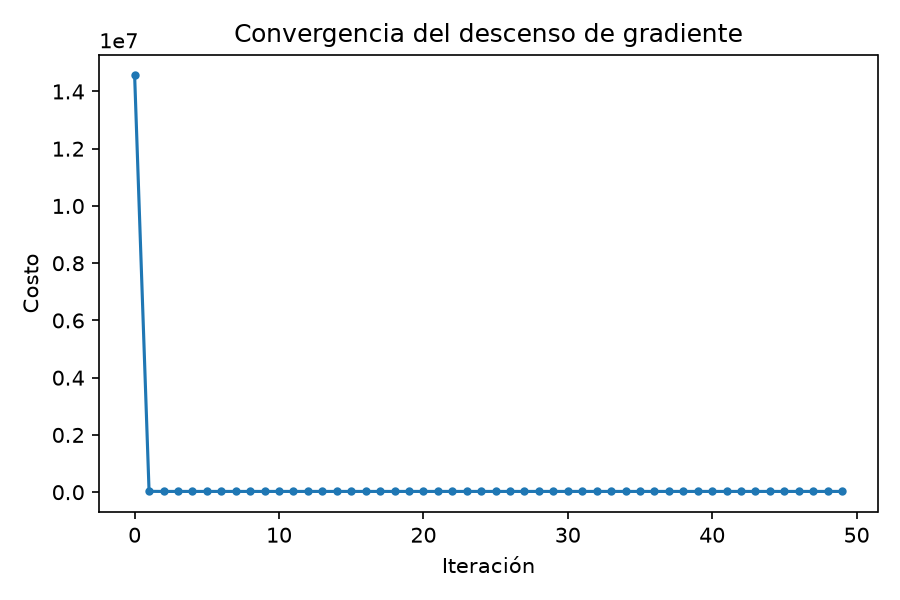
\includegraphics[width=\columnwidth]{convergencia_verificacion_lineal.png}
    \caption{Convergencia del descenso de gradiente en la prueba de verificación.}
    \label{fig:convergencia_verificacion_lineal}
\end{figure}

La curva de costo decrece de forma monótona y se estabiliza, lo que confirma que la implementación es correcta y numéricamente estable.

\subsection{Experimentación}
Se comparan tres hipótesis de complejidad creciente, evaluadas siempre con el error de validación:
\begin{itemize}
    \item \textbf{Modelo A:} únicamente variables numéricas originales.
    \item \textbf{Modelo B:} Modelo A más variables categóricas como variables dummy.
    \item \textbf{Modelo C:} Modelo B más términos polinómicos cuadráticos de variables climáticas relevantes.
\end{itemize}

Sobre el Modelo C, y utilizando la tasa de aprendizaje $\alpha=0.05$ ya validada, se prueban distintos valores de $\lambda$ para obtener el Modelo D, comparando el RMSE de validación de cada configuración y eligiendo el valor que lo minimiza.

\begin{table}[h]
\centering
\caption{Comparación de RMSE por hipótesis sobre el conjunto de validación.}
\label{tab:rmse_modelos}
\begin{tabular}{@{}lcc@{}}
\toprule
\textbf{Modelo} & \textbf{RMSE train} & \textbf{RMSE val} \\
\midrule
A: numéricas & 226.48 & 210.53 \\
B: más categóricas & 225.40 & 210.55 \\
C: más polinomios & 225.40 & 210.55 \\
D: Ridge & 225.40 & 210.55 \\
\bottomrule
\end{tabular}
\end{table}

El barrido de valores de $\lambda$ sobre el Modelo C selecciona $\lambda=0.0$ como óptimo, ya que valores mayores solo incrementan el RMSE de validación. El Modelo D se entrena entonces con $\alpha=0.05$ y $\lambda=0.0$.

\subsection{Evaluación final}
Una vez seleccionado el Modelo D con el conjunto de validación, se evalúa una única vez sobre el conjunto de test. El modelo obtiene un RMSE de test de $228.09$ Kg por hectárea, frente a una desviación estándar de la productividad de $283.24$ Kg por hectárea y una media de $5990.53$ Kg por hectárea.

\subsection{Análisis de resultados y conclusiones}
El error del modelo final es considerablemente menor que la variabilidad natural de la productividad, lo que indica una mejora real sobre predecir siempre la media, aunque sin llegar a un ajuste muy alto.

Estandarizar las variables utilizando únicamente los estadísticos del conjunto de entrenamiento resultó indispensable para la convergencia del descenso de gradiente. Detectar y eliminar variables redundantes antes de modelar también fue una decisión metodológica clave, y se verificó que eliminarlas no empeora el desempeño de validación ni de test, lo que confirma que no aportaban señal adicional relevante.

Agregar variables categóricas produjo una mejora pequeña pero consistente sobre el error de validación del Modelo A. En contraste, los términos polinómicos del Modelo C no mejoraron el error de validación frente al Modelo B, lo que sugiere que la relación entre las variables climáticas disponibles y la productividad no es fuertemente no lineal, sino una señal débil distribuida entre muchos factores agroclimáticos.

La regularización L2 tampoco aportó una mejora adicional, ya que el barrido de $\lambda$ seleccionó $\lambda=0.0$ como óptimo. Esto es consistente con que, una vez eliminadas las variables redundantes, el modelo ya no presenta una multicolinealidad severa que penalizar.

El dataset probablemente mezcla parcelas con prácticas de manejo no observadas, lo que limita el techo de desempeño alcanzable con un modelo lineal, y un modelo de esta naturaleza puede estar subestimando interacciones más complejas entre variables climáticas y agronómicas.

%======================================================================
% ===================== PUNTO 2 (COMPLETO) ============================
%======================================================================
\section{Punto 2: Regresión Logística}

\subsection{Exploración de datos}

\subsubsection{Limpieza}
Se realiza una limpieza inicial sobre la variable objetivo \texttt{Variety}. Se eliminan los registros correspondientes a la variedad \emph{delux ponni}, dado que el problema se plantea como una \textbf{clasificación binaria} y se trabaja únicamente con las variedades \emph{ponmani} y \emph{CO\_43}. Posteriormente, la variable categórica \texttt{Variety} se transforma a valores numéricos de la siguiente manera:
\begin{itemize}
    \item \emph{ponmani} $\rightarrow 0$
    \item \emph{CO\_43} $\rightarrow 1$
\end{itemize}
Esta transformación permite utilizar \texttt{Variety} como variable objetivo binaria dentro del modelo de regresión logística.

\subsubsection{Correlación}
Se calcula la correlación entre cada variable predictora numérica y la variable objetivo \texttt{Variety}, con el propósito de identificar qué variables presentan mayor relación lineal con la clase a predecir. Los resultados muestran que la mayoría de las variables presentan una correlación cercana a cero, y la variable con mayor correlación en valor absoluto es \texttt{Trash(in bundles)}, con aproximadamente $-0.13$.

\begin{figure}[h]
    \centering
    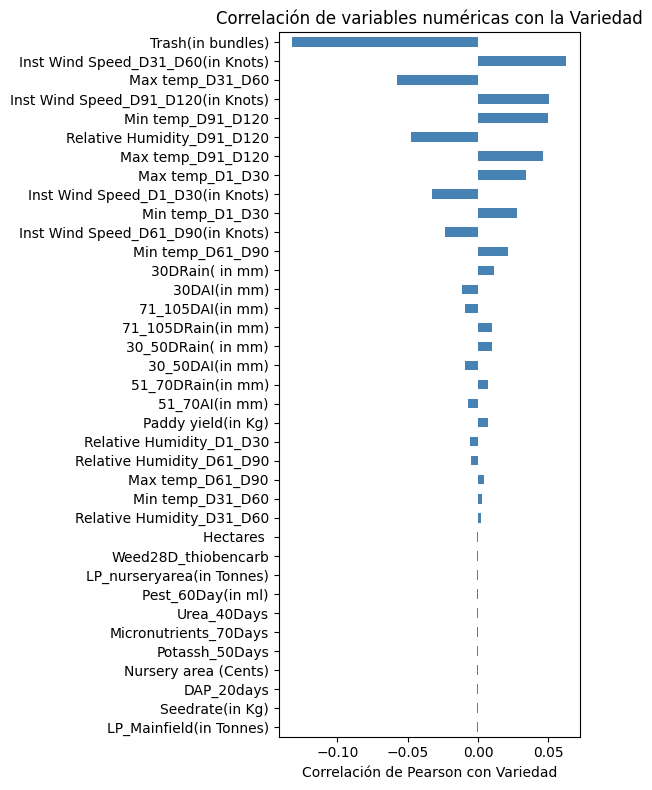
\includegraphics[width=\columnwidth]{correlacion_variety.png}
    \caption{Correlación de Pearson de las variables numéricas con la variable objetivo \texttt{Variety}.}
    \label{fig:correlacion_variety}
\end{figure}
% Nombre de imagen sugerido: correlacion_variety.png  (celda 59 del notebook)

\paragraph{Identificación de variables redundantes}
Al analizar la correlación entre algunas variables agrícolas se observa que presentan una correlación de $1.0$ entre sí, lo que indica que contienen información completamente redundante. Por esta razón se eliminan las variables:
\begin{itemize}
    \item \texttt{Seedrate(in Kg)}
    \item \texttt{LP\_Mainfield(in Tonnes)}
    \item \texttt{Nursery area (Cents)}
    \item \texttt{LP\_nurseryarea(in Tonnes)}
    \item \texttt{DAP\_20days}
\end{itemize}
conservando \texttt{Hectares} como representante de este grupo altamente correlacionado.

\subsubsection{Transformación}
Se transforman las variables categóricas y las relacionadas con la dirección del viento para que puedan ser utilizadas correctamente por el modelo de regresión logística. La dirección del viento (\texttt{N}, \texttt{NE}, \texttt{S}, \texttt{SW}, etc.) es una variable de naturaleza \emph{circular}: por ejemplo, \texttt{N} y \texttt{NNW} están próximas entre sí, relación que una codificación numérica convencional no capturaría correctamente. Por ello, cada dirección se convierte primero a grados ($\theta$) y luego se codifica mediante seno y coseno:

\begin{equation}
x_{\sin} = \sin(\theta)
\label{eq:wind_sin}
\end{equation}

\begin{equation}
x_{\cos} = \cos(\theta)
\label{eq:wind_cos}
\end{equation}

De esta manera se conserva la naturaleza circular de la dirección del viento. Las demás variables categóricas se convierten mediante \textbf{One-Hot Encoding}, utilizando \texttt{drop\_first=True} para eliminar una categoría de referencia por variable y evitar colinealidad perfecta con el término de sesgo.

\subsection{Partición de datos}
Se separan las variables predictoras $X$ de la variable objetivo $y$, donde \texttt{Variety} representa la clase a predecir. El conjunto de datos se divide en tres subconjuntos, utilizando \texttt{random\_state=200} para garantizar reproducibilidad:
\begin{itemize}
    \item \textbf{Train (70\%):} para ajustar los parámetros del modelo.
    \item \textbf{Validation (15\%):} para comparar configuraciones y seleccionar el mejor modelo.
    \item \textbf{Test (15\%):} reservado para la evaluación final, usado una única vez.
\end{itemize}

\subsection{Implementación del modelo}

Se implementa manualmente el entrenamiento de una regresión logística mediante \textbf{descenso de gradiente}. El modelo calcula inicialmente una combinación lineal de las características:

\begin{equation}
z = X\theta
\label{eq:linear_combination}
\end{equation}

donde $X$ es la matriz de características (con la columna de sesgo incluida), $\theta$ son los parámetros del modelo y $z$ es la combinación lineal resultante.

Para convertir esta combinación lineal en una probabilidad se utiliza la función sigmoide:

\begin{equation}
\sigma(z) = \frac{1}{1+e^{-z}}
\label{eq:sigmoid}
\end{equation}

Por lo tanto, la probabilidad estimada de pertenecer a la clase 1 es:

\begin{equation}
\hat{y} = \sigma(X\theta)
\label{eq:yhat}
\end{equation}

\subsubsection{Función de costo}
El error del modelo se mide mediante \textbf{Log-Loss}:

\begin{equation}
J(\theta) = -\frac{1}{n}\sum_{i=1}^{n}\left[y_i\log(\hat{y}_i) + (1-y_i)\log(1-\hat{y}_i)\right]
\label{eq:logloss}
\end{equation}

Esta función penaliza fuertemente las predicciones que asignan una probabilidad incorrecta a la clase real. Adicionalmente, el modelo incorpora regularización L2:

\begin{equation}
J_{reg}(\theta) = J(\theta) + \frac{\lambda}{2n}\sum_{j=1}^{m}\theta_j^2
\label{eq:logloss_reg}
\end{equation}

La regularización evita que los pesos del modelo tomen valores excesivamente grandes. El término correspondiente al sesgo ($\theta_0$) nunca se regulariza.

\subsubsection{Actualización de los parámetros}
El gradiente de la función de costo se calcula Con regularización:

\begin{equation}
\nabla J_{reg}(\theta) = \frac{1}{n}X^\top(\hat{y}-y) + \frac{\lambda}{n}\theta
\label{eq:grad_reg}
\end{equation}

sin aplicar la penalización al término de sesgo. Finalmente, los parámetros se actualizan mediante descenso de gradiente:

\begin{equation}
\theta := \theta - \alpha\nabla J_{reg}(\theta)
\label{eq:update}
\end{equation}

donde $\alpha$ es la tasa de aprendizaje, que determina el tamaño de cada paso de la optimización. El proceso se repite durante el número de épocas establecido, almacenando el costo periódicamente para analizar la convergencia del algoritmo.

\subsection{Verificación de la implementación}
Antes de utilizar el modelo completo, se realiza una prueba controlada utilizando únicamente la variable \texttt{Hectares}. El objetivo de esta etapa no es obtener el mejor clasificador, sino verificar que la implementación del descenso de gradiente funciona correctamente.

Primero se estandariza la variable:

\begin{equation}
x' = \frac{x-\mu}{\sigma}
\label{eq:standardize}
\end{equation}

y posteriormente se agrega el término de sesgo para que el modelo pueda aprender el intercepto. Se entrena el modelo durante 2000 épocas, con una tasa de aprendizaje $\alpha = 0.1$ y una regularización $\lambda = 0.05$.

\begin{figure}[h]
    \centering
    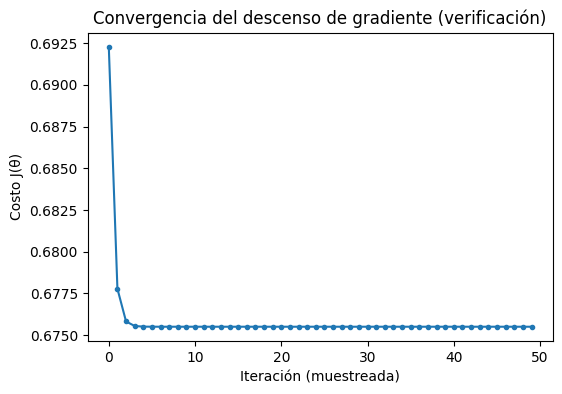
\includegraphics[width=\columnwidth]{convergencia_verificacion_logistica.png}
    \caption{Convergencia del descenso de gradiente en la prueba de verificación (modelo con únicamente \texttt{Hectares}).}
    \label{fig:convergencia_verificacion}
\end{figure}
% Nombre de imagen sugerido: convergencia_verificacion_logistica.png (celda 76 del notebook)

La curva de costo confirma que el algoritmo converge de forma decreciente.

\subsection{Evaluación del modelo de verificación}
Una vez entrenado el modelo de prueba, se calculan las probabilidades predichas mediante la función sigmoide (Ec.~\ref{eq:sigmoid}). Para convertir estas probabilidades en clases se utiliza un umbral de $0.5$:

\begin{equation}
\hat{y} =
\begin{cases}
1 & \text{si } P(y=1|x)\geq 0.5\\
0 & \text{si } P(y=1|x)< 0.5
\end{cases}
\label{eq:threshold}
\end{equation}

Posteriormente se construye la matriz de confusión y se calculan Accuracy, Precision, Recall y F1-score. En esta prueba, el modelo predice todos los registros como clase 0, lo que genera un \textbf{Accuracy de aproximadamente 59.36\%}, pero Precision, Recall y F1-score para la clase 1 son iguales a cero. Este resultado muestra que, aunque el algoritmo de optimización converge correctamente, utilizar únicamente \texttt{Hectares} no proporciona suficiente información para distinguir adecuadamente entre las dos variedades.

\subsection{Construcción progresiva de las hipótesis}
Para estudiar cómo influye la selección de variables en el desempeño del modelo, se plantearon inicialmente diferentes modelos de forma progresiva (M1 a M5, de menor a mayor cantidad de variables). Durante la evaluación se encontró un comportamiento inesperado: al combinar \texttt{Trash(in bundles)} con cualquiera de las variables agrícolas se obtenía un desempeño del \textbf{100\%}. Este resultado se consideró una señal de alerta, ya que un desempeño perfecto puede indicar redundancia, una relación extremadamente fuerte entre variables o incluso fuga de información.

Por esta razón, se modificó la estrategia de construcción de modelos para estudiar por separado el efecto de \texttt{Trash} y evitar que su combinación con las variables agricolas, se realizó las siguientes configuraciones:

\begin{itemize}
    \item \textbf{M1:} Todas las variables, excepto \texttt{Trash(in bundles)}.
    \item \textbf{M2:} Únicamente \texttt{Trash(in bundles)}.
    \item \textbf{M3:} Todas las variables, excluyendo las variables agrícolas, más \texttt{Trash}.
    \item \textbf{M4:} Subconjunto reducido de variables con mayor correlación observada con \texttt{Variety}.
\end{itemize}

Para cada configuración se realizó una búsqueda de hiperparámetros sobre una grilla de tasas de aprendizaje $\alpha \in \{0.001, 0.01, 0.1\}$, número de épocas $\in \{1000, 2000, 5000\}$ y coeficientes de regularización $\lambda \in \{0.0, 0.01, 0.05, 0.1, 1.0\}$, evaluando siempre sobre el conjunto de validación.

\subsection{Selección del mejor modelo y evaluación en test}
Después de entrenar y evaluar las diferentes configuraciones, se compararon sus resultados utilizando las métricas de clasificación. El modelo seleccionado fue \textbf{M3}, con los siguientes hiperparámetros:
\begin{itemize}
    \item $\alpha = 0.1$
    \item Épocas $= 5000$
    \item $\lambda = 0.0$
\end{itemize}

En el conjunto de validación obtuvo:
\begin{itemize}
    \item Accuracy: \textbf{89.96\%}
    \item Precision: \textbf{94.38\%}
    \item Recall: \textbf{79.25\%}
    \item F1-score: \textbf{86.15\%}
\end{itemize}

Una vez seleccionado M3 utilizando el conjunto de validación, se realizó la evaluación final utilizando exclusivamente el conjunto de \textbf{test}. El modelo final obtuvo:
\begin{itemize}
    \item Accuracy: \textbf{89.96\%}
    \item Precision: \textbf{94.06\%}
    \item Recall: \textbf{81.90\%}
    \item F1-score: \textbf{87.56\%}
    \item Log-loss: \textbf{0.3502}
\end{itemize}

\begin{table}[h]
\centering
\caption{Matriz de confusión del modelo M3 sobre el conjunto de test.}
\label{tab:confusion_matrix}
\begin{tabular}{@{}lcc@{}}
\toprule
 & \textbf{Predicción 0} & \textbf{Predicción 1} \\
\midrule
\textbf{Real 0} & 147 & 6 \\
\textbf{Real 1} & 21  & 95 \\
\bottomrule
\end{tabular}
\end{table}

El modelo clasifica correctamente la gran mayoría de los registros de ambas clases. En particular, se observan pocos falsos positivos (6), mientras que se presentan 21 falsos negativos. El Accuracy cercano al 90\% y el F1-score de aproximadamente 0.876 indican un buen desempeño general en el conjunto de prueba. La comparación entre validación y test también muestra resultados similares, lo que constituye una señal favorable de que el modelo mantiene su capacidad predictiva sobre datos no utilizados durante el entrenamiento.

\subsection{Análisis de resultados y conclusiones}

La implementación del modelo de regresión logística demuestra que la calidad predictiva depende fundamentalmente de una rigurosa curación de los datos. La exclusión temprana de variables altamente colineales y el tratamiento cuidadoso de \texttt{Trash(in bundles)} resultaron ser decisiones críticas para evitar la fuga de información.

Por otro lado, el modelo final (\textbf{M3}) exhibe una sólida capacidad de generalización, manteniendo un \emph{Accuracy} del 89.96\% en el conjunto de prueba, sin caídas drásticas respecto a la validación. El balance entre su \emph{Precision} (94.06\%) y \emph{Recall} (81.90\%) revela un clasificador estricto que es sumamente preciso al predecir la clase positiva, minimizando la tasa de falsos positivos a cambio de permitir algunos falsos negativos.

\begin{thebibliography}{1}
\bibitem{b1} UCI Machine Learning Repository, ``Paddy Dataset,'' \emph{archive.ics.uci.edu}, 2024. [Online]. Available: https://archive.ics.uci.edu/dataset/1186/paddy+dataset
\end{thebibliography}

\end{document}
